\documentclass{beamer}
\usetheme{metropolis}
\usepackage{graphicx}
\usepackage{booktabs}
\usepackage{hyperref}
\usepackage{listings}
\colorlet{shadecolor}{gray!40}

\lstset{
	language=R,
	basicstyle=\ttfamily\small,
	commentstyle=\color{black},
	keywordstyle=\color{blue},
	numbers=left,
	numberstyle=\tiny\color{red},
	stepnumber=1,
	numbersep=5pt,
	backgroundcolor=\color{shadecolor},
	showspaces=false,
	showstringspaces=false,
	showtabs=false,
	frame=single,
	tabsize=2,
	captionpos=b,
	breaklines=true,
	breakatwhitespace=false,
	title=\lstname
}


\newenvironment{bigitemize}{\itemize\addtolength{\itemsep}{10pt}}{\enditemize}
\newcommand\independent{\protect\mathpalette{\protect\independenT}{\perp}}
\def\independenT#1#2{\mathrel{\rlap{$#1#2$}\mkern2mu{#1#2}}}
\title{Microeconometrics Module}
\subtitle{Lecture 5: Randomized Control Trials}
\author{Swapnil Singh}
\date{Lietuvos Bankas and KTU \\ \href{https://github.com/swapnil1987/econometrics-2024}{\textcolor{magenta}{Course Link}}}

\begin{document}
	
	\maketitle
	
	\begin{frame}
		\frametitle{Randomization}
		\begin{itemize}
			\item Through randomization we can remove selection bias
			\item The idea of randomization
			\begin{itemize}
				\item Select a group of people who are uninsured
				\item Randomly provide some people health insurance (treatment group)
				\item Other individuals don't receive insurance (control group)
				\item Due to law of large number, we will be comparing apples with apples
			\end{itemize}
		\end{itemize}
	\end{frame}
	
	\begin{frame}
		\frametitle{Selection Bias Elimination}
		\begin{itemize}
			\item Due to law of large numbers
			$$ \mathbb E[Y_{0i} | D_i = 1] = \mathbb E[Y_{0i} | D_i = 0] $$
			\item Notice the change from $Avg_n$ to $\mathbb E$
			\item Hence we can write following equations
			\begin{align*}
				&\Rightarrow \mathbb E[Y_i | D_i = 1] - \mathbb E[Y_i | D_i = 0]\\
				&\Rightarrow \mathbb E[Y_{1i} | D_i = 1] - \mathbb E[Y_{0i} | D_i = 0]\\
				&\Rightarrow \mathbb E[\kappa + Y_{0i} | D_i = 1] - \mathbb E[Y_i | D_i = 0]\\
				&\Rightarrow \kappa + \underbrace{E[Y_{0i} | D_i = 1] - \mathbb E[Y_i | D_i = 0]}_{= 0}\\
				&= \kappa
			\end{align*}
			\item Note that randomization does not work because we eliminate individual differences
			\item It works because law of large number makes sure that on average, mix of individuals is same
		\end{itemize}
	\end{frame}
	
	\begin{frame}
		\frametitle{RAND Health Insurance Experiment (HIE)}
		\begin{itemize}
			\item HIE ran from 1974 to 1982
			\item 3,958 people age 14 to 61 were enrolled
			\item People who had some type of insurance before hand were excluded
			\item Participants were assigned to one of 14 insurance plans
			\item Plans had provision for cost sharing, creating large differences in the amount of insurance offered
			\item Most generous: comprehensive care for free
			\item Least generous: families had to pay 95 percent of their health care costs
			\item Among all plans, catastrophic plans provide control group
			\item Other plans provide treatment group
		\end{itemize}
	\end{frame}
	
	\begin{frame}
		\frametitle{HIE Results}
		\begin{figure}
			\centering
			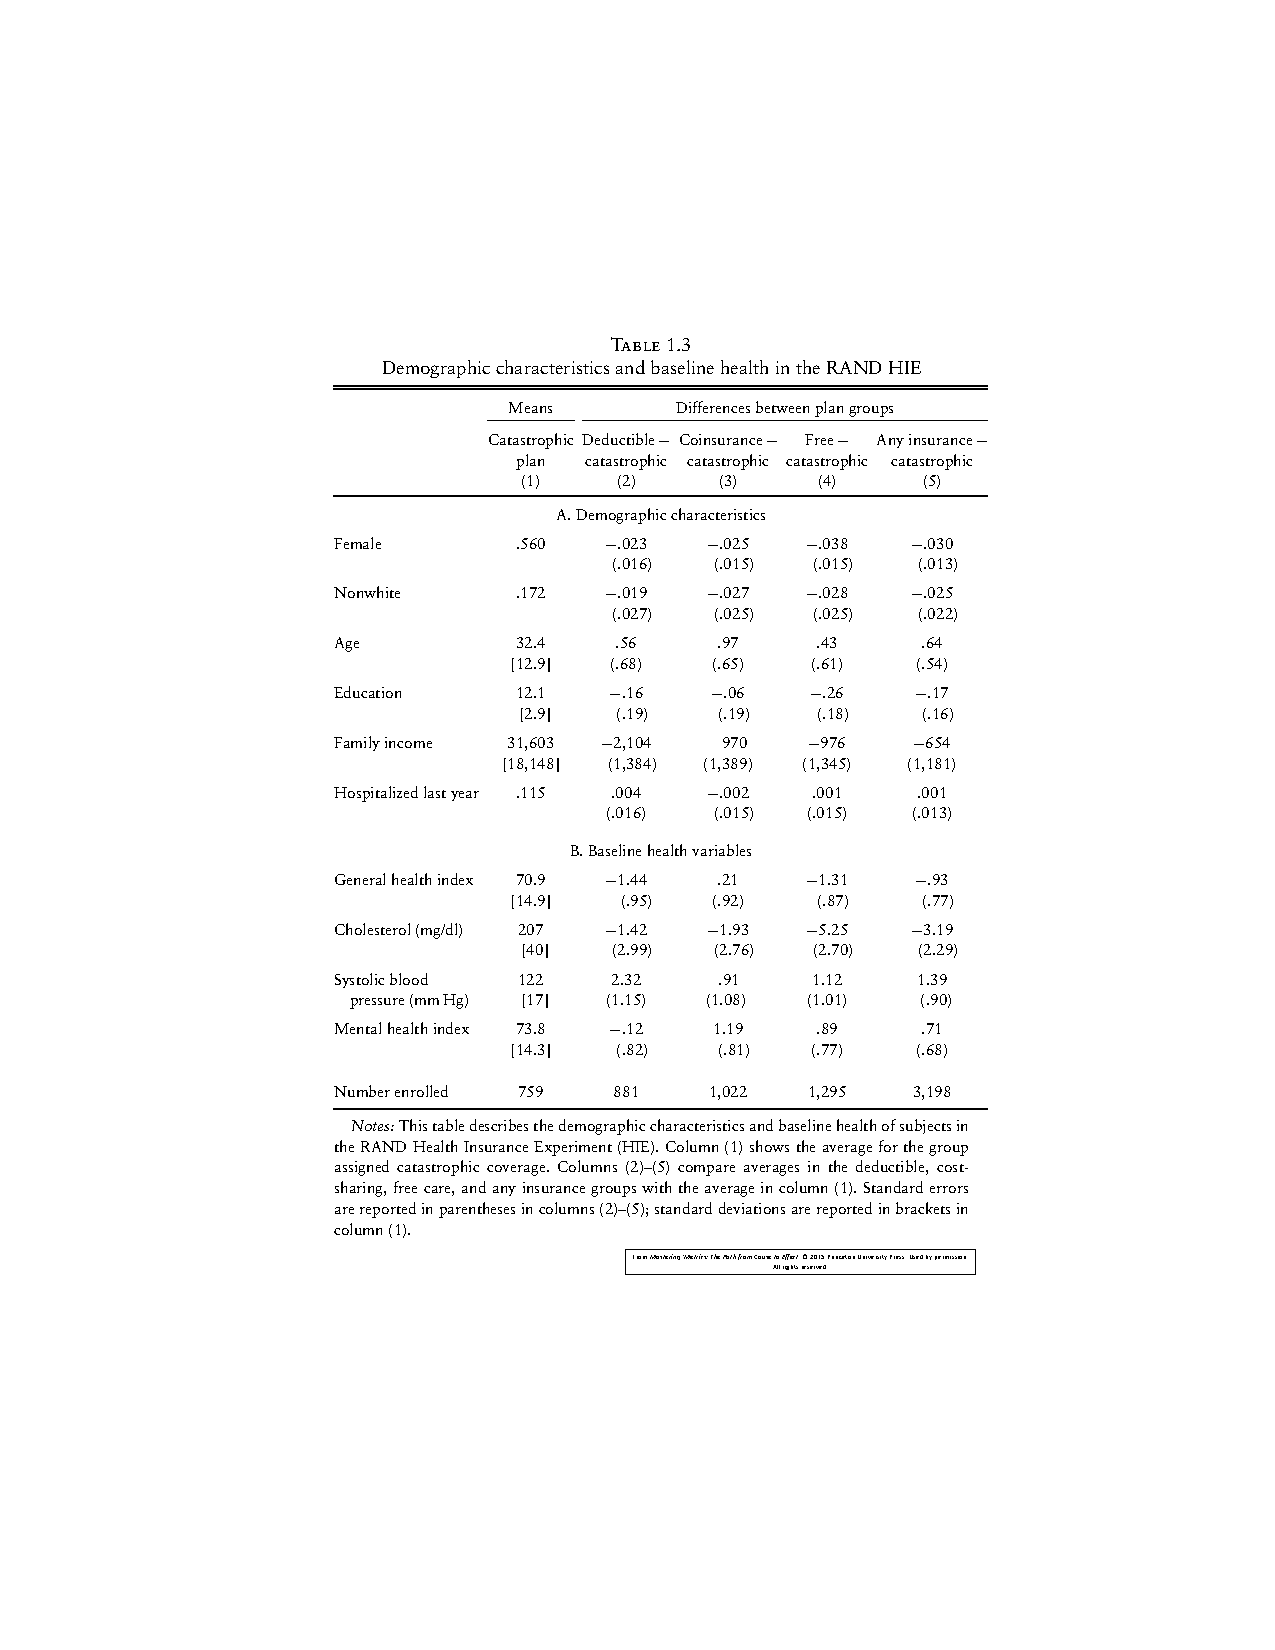
\includegraphics[ height=\textheight]{Figures/MMtbl13}
		\end{figure}
	\end{frame}
	
	\begin{frame}
		\frametitle{HIE Results}
		\begin{figure}
			\centering
			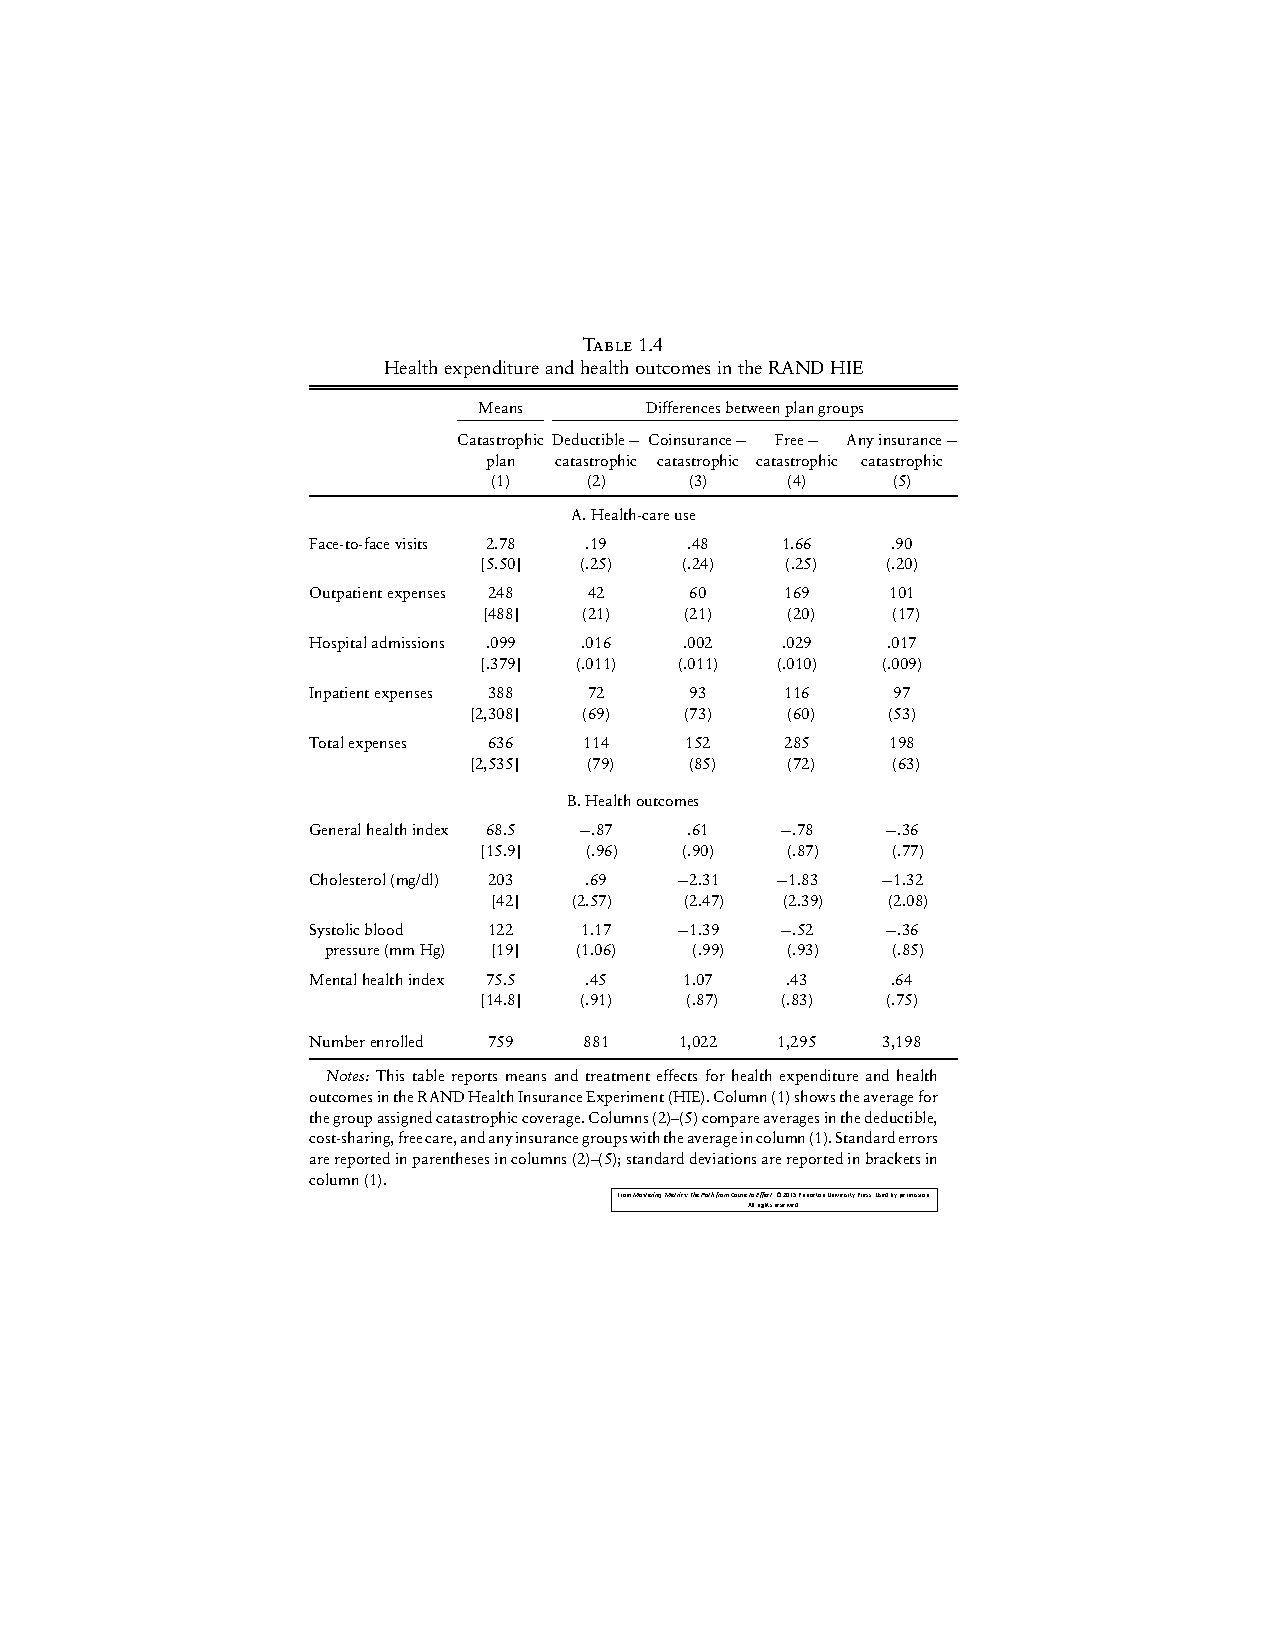
\includegraphics[ height=\textheight]{Figures/MMtbl14}
		\end{figure}
	\end{frame}
	
	\begin{frame}
		\frametitle{Oregon Experiment}
		\begin{itemize}
			\item Expansion of Medicaid offering in Oregon
			\item Oregon issued health insurance lottery
			\item Individuals were randomly selected to get health care insurance
			\item Some numbers:
			\begin{itemize}
				\item 75,000 registered for Oregon Health Plan (OHP)
				\item 30,000 won and became treatment group
				\item 45,000 lost and became control group
			\end{itemize}
			\item There were some minor changes down the line. Not important for the exposition right now
		\end{itemize}
	\end{frame}
	
	\begin{frame}
		\frametitle{Oregon Experiment Results}
		\begin{figure}
			\centering
			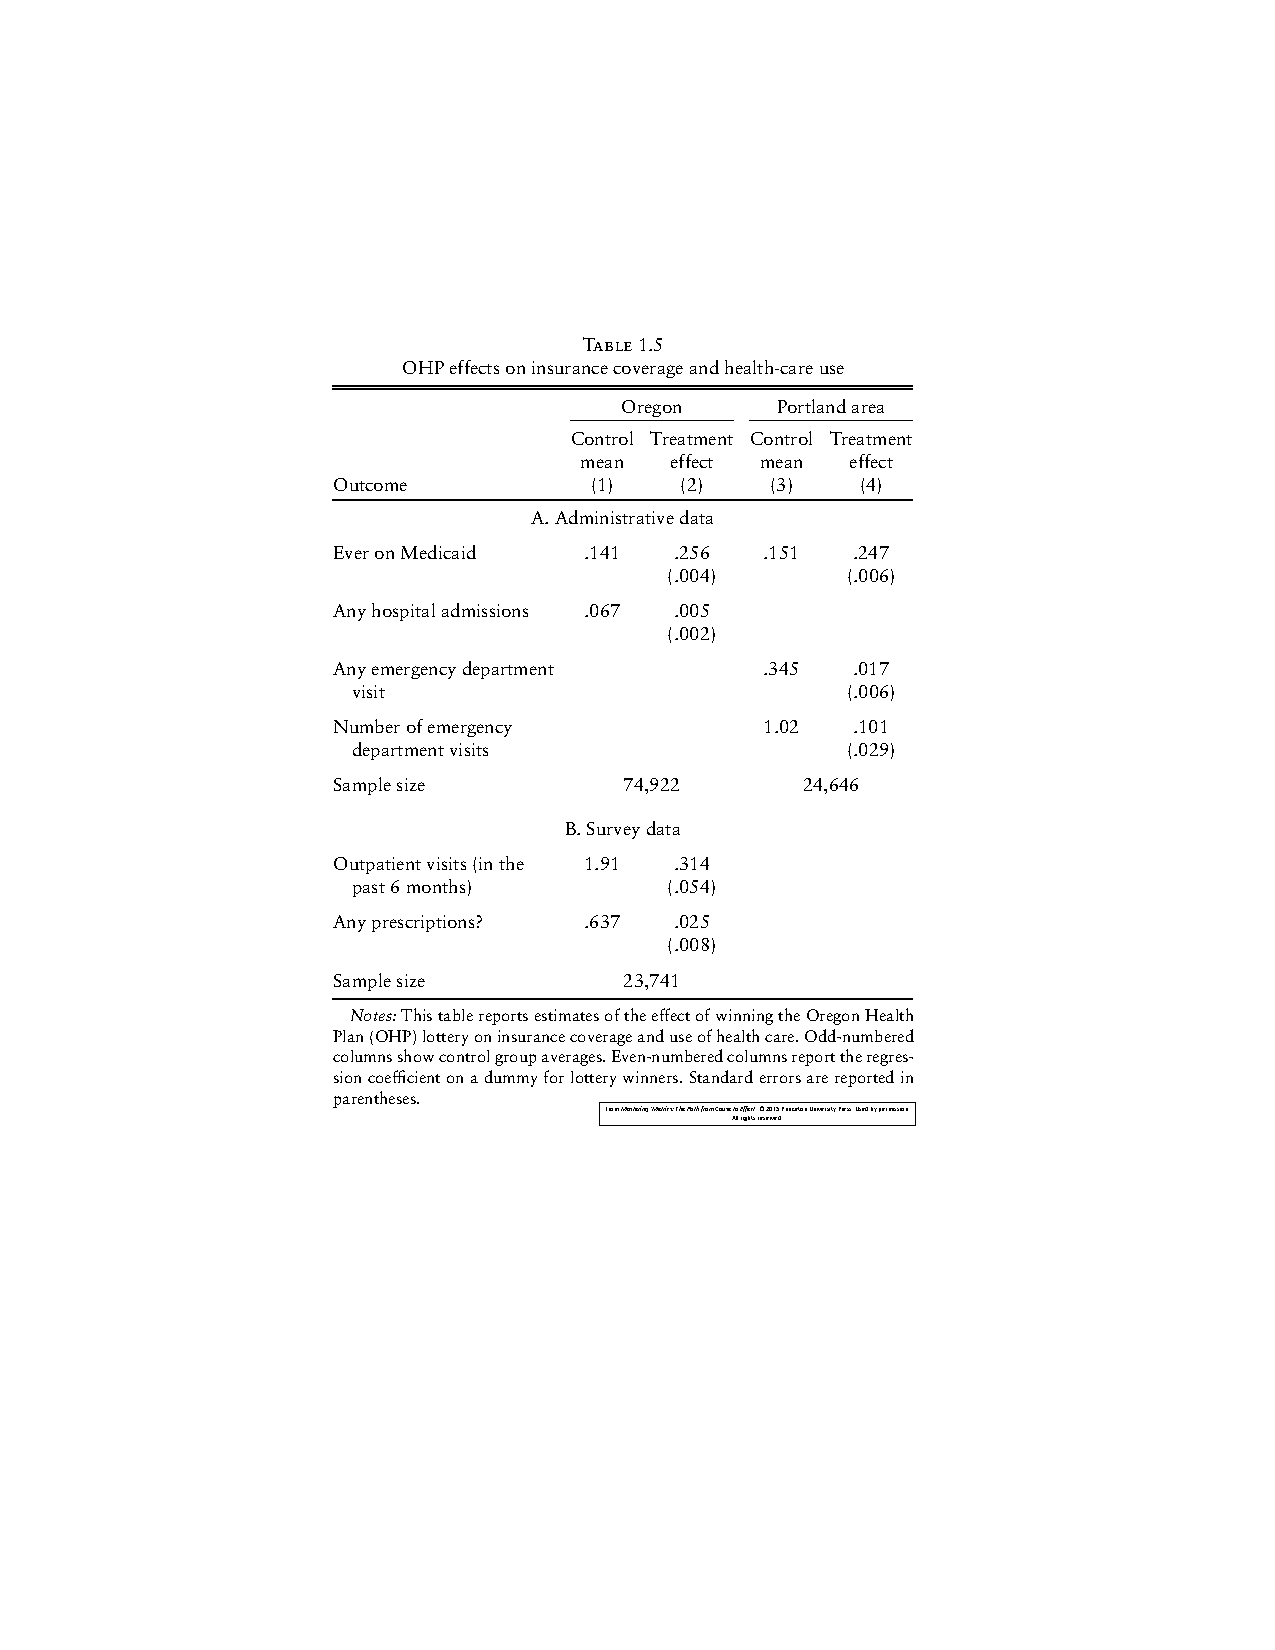
\includegraphics[ height=\textheight]{Figures/MMtbl15}
		\end{figure}
	\end{frame}
	
	\begin{frame}
		\frametitle{Oregon Experiment Results}
		\begin{figure}
			\centering
			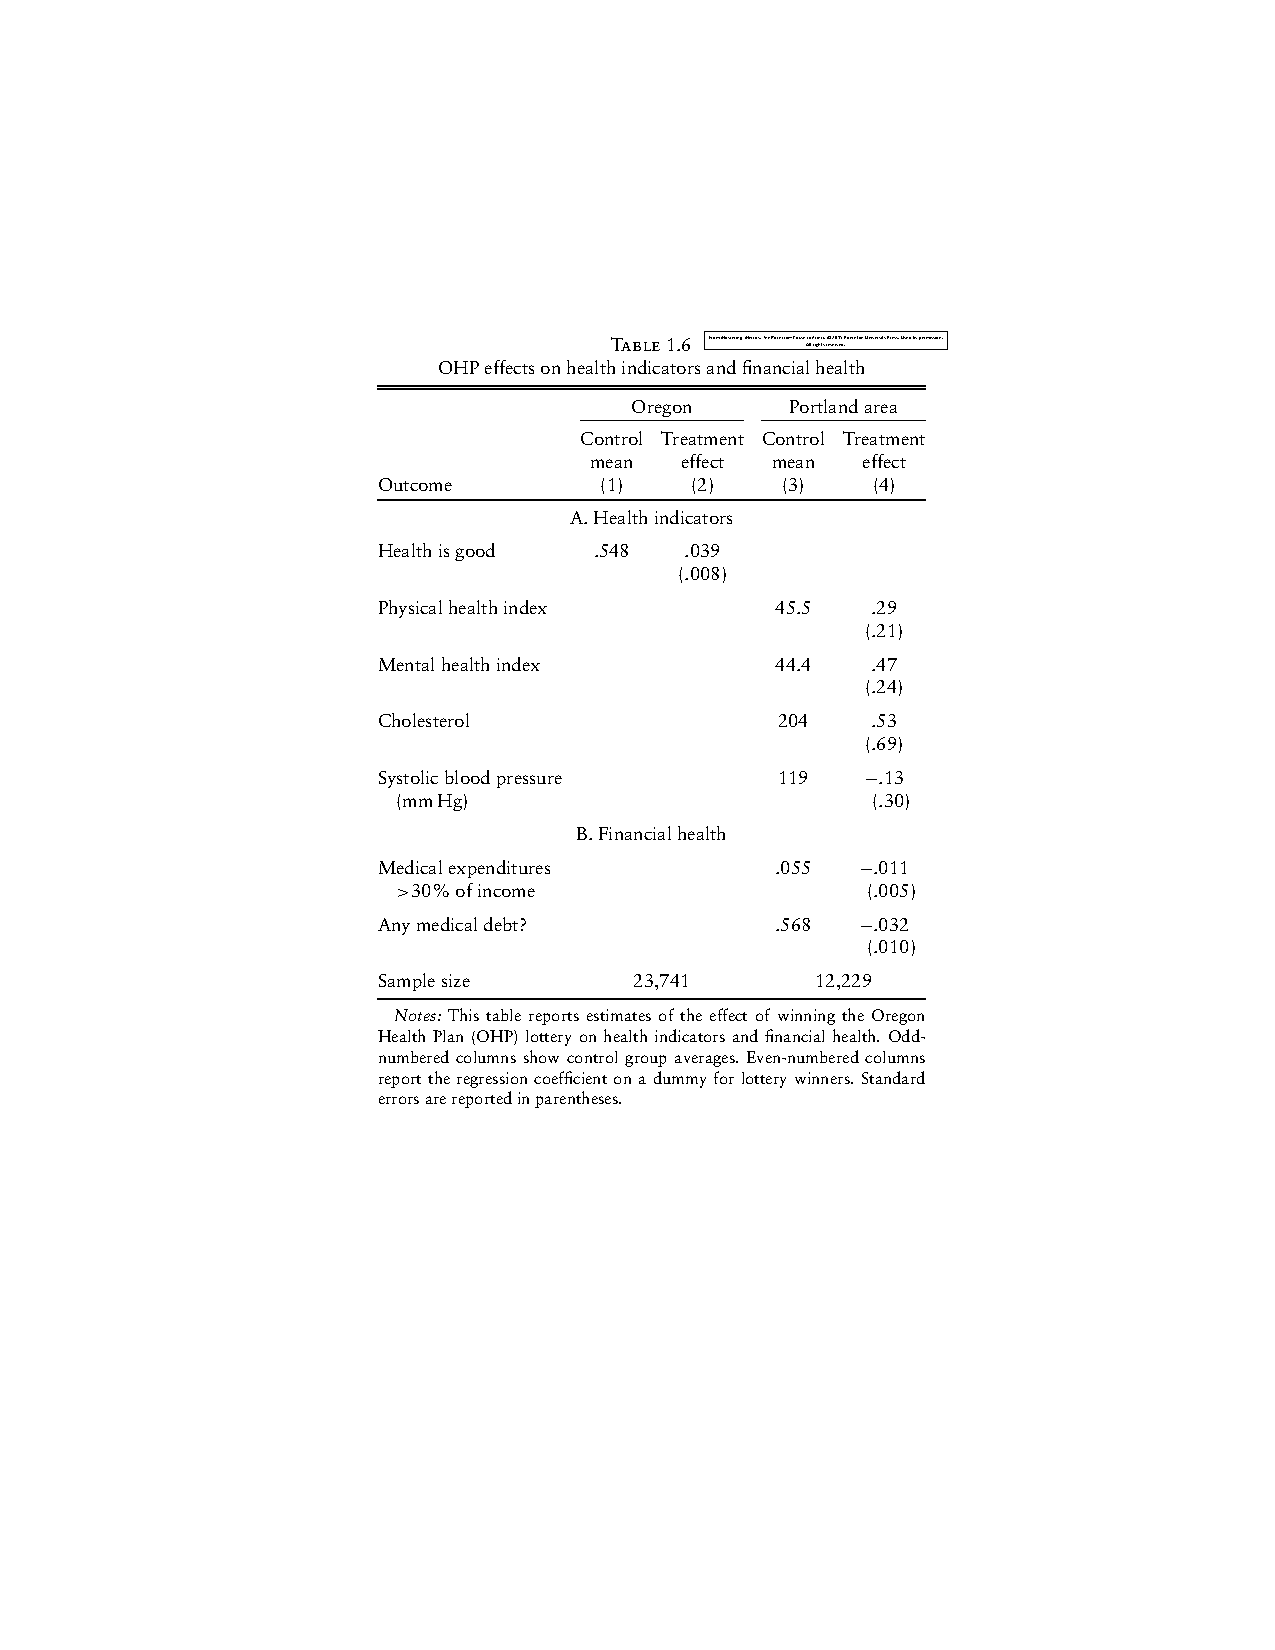
\includegraphics[ height=\textheight]{Figures/MMtbl16}
		\end{figure}
	\end{frame}
	
	\begin{frame}
		\frametitle{Quick Recap}\label{back_appendix_rct}
		\begin{itemize}
			\item Causal inference means comparing potential outcomes
			\item However, selection bias makes our life difficult
			\item We discuss how randomization can actually eliminate selection bias
			\begin{itemize}
				\item The catch here is checking for balance: whether law of large number does its magic or not
			\end{itemize}
			
		\end{itemize}
	\end{frame}
	
	
\end{document}